\chapter{Marco Teórico}
\section{Conceptos de Visión}

\subsection{Visión Humana}
De una manera muy generar, vision se entiendo como toda accion de ver, sin embargo, desde un punto de vista mas tecnico, vision es la capacidad de interpretar nuestro entorno gracias a los rayos de luz que alcanzan el ojo. Otros autores definen vision como una capacidad necesaria mas no impresindible para realizar las actividades cotidianas.

Desde el punto de la vista de la medicina, la visión humana o sentido de la vista se reduce a un organo receptor conocido como el \textit{ojo}, la membrana y retina son los encargados de recivir las impresiones luminosas para luego transmitirlas al cerebro por medio de las vias opticas(ver figura~\ref{fig:estructura_percepcion}). En adicion, el ojo es un organo situado en la cavidad orbitaria, esta protegida por los parpados y por la secrecion de las glandulas lagrumales. Los ojos son sensibles a ondas de radiación electromagnética de longitudes específicas. Estas ondas se registran como la sensación de la luz. Cuando la luz penetra en el ojo, pasa a través de la córnea, la pupila y el cristalino, y llega por último a la retina, donde la energía electromagnética de la luz se convierte en impulsos nerviosos que pueden ser utilizados por el cerebro. Los impulsos abandonan el ojo a través del nervio
óptico. La región más sensible del ojo en la visión normal diurna es una pequeña depresión de la retina llamada fóvea en el cual se enfoca la luz que viene del centro del campo visual (por campo visual entendemos aquello a lo que mira el sujeto). Puesto que la lente simple convexa invierte la imagen, el campo visual derecho es representado a la izquierda de la retina y el campo inferior representado en lo alto de la retina. El ojo es un sistema óptico muy imperfecto. Las ondas de luz no solo tienen que pasar a través de los humores y el cristalino, después penetrar la red de los vasos sanguíneos y fibras nerviosas antes de que lleguen las células sensibles los bastones y los conos de la retina donde la luz se convierte en impulsos nerviosos. A pesar de estas imperfecciones el ojo funciona muy bien. La fóvea es capaz de percibir un cable telefónico a 400 m de distancia. En buenas condiciones el ojo puede percibir un alambre cuyo grosor no cubre más de 0,5 mm.

Tambien exister otras definiciones que indican que, el ojo es la puerta de entrada por la que ingresan los estímulos luminosos que se transforman en impulsos eléctricos gracias a unas células especializadas de la retina que son los conos y los bastones. Entonces, el nervio óptico transmite los impulsos eléctricos generados en la retina al cerebro, donde son procesados en la corteza visual. Finalmente, en el cerebro tiene lugar el complicado proceso de la percepción visual gracias al cual somos capaces de percibir la forma de los objetos, identificar distancias, detectar los colores y el movimiento~\cite{14alonso2005personas}.


        \begin{figure}[H]
		\centering
		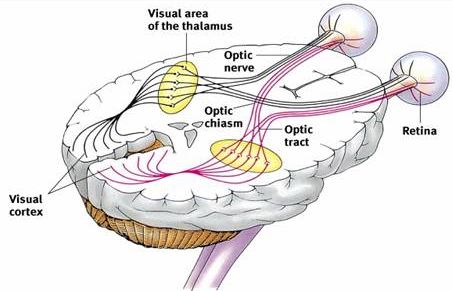
\includegraphics[width=100mm]{Imagenes/estructura_percepcion.jpg}
		\caption{Estructura de la percepción visual humana.}
		\vspace{0.15cm}
		\textit{Fuente: Fernando Vila Arroyo, “El Libro Blanco de la Iluminación”. España 2013.}
		\label{fig:estructura_percepcion}
		\end{figure}      	  

\subsection{Visión por Computador}
La visión artificial o también conocida como visión por computador es una disciplina científica que incluye métodos para adquirir, procesar, analizar y comprender las imágenes del mundo real con el fin de producir información numérica o simbólica para que puedan ser tratados por un computador. Tal y como los humanos usamos nuestros ojos y cerebros para comprender el mundo que nos rodea, la visión por computador trata de producir el mismo efecto para que las computadoras puedan percibir y comprender una imagen o secuencia de imágenes y actuar según convenga en una determinada situación. Esta comprensión se consigue gracias a distintos campos como la geometría, la estadística, la física y otras disciplinas. La adquisición de los datos se consigue por varios medios como secuencias de imágenes, vistas desde varias cámaras de video o datos multidimensionales desde un
escáner médico.

Hay muchas tecnologías que utilizan la visión por computador(figura~\ref{fig:esquema_vision_computador}), entre las cuáles tenemos: reconocimiento de objetos, detección de eventos, reconstrucción de una escena (\textit{mapping}) y restauración de imágenes~\cite{15VC}.


\begin{figure}[H]
		\centering
		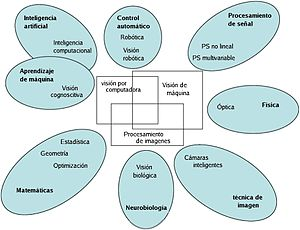
\includegraphics[width=100mm]{./Imagenes/esquema_vision_computador.jpg}
		\caption{Esquema de las relaciones entre la visión por computadora y otras áreas afines.}
		\vspace{0.15cm}
		\textit{Fuente: Visión artificial, Wikipedia.}
		\label{fig:esquema_vision_computador}
\end{figure}  


\section{Deteccion de Rostros}
En los ultimos años investigadores de todo el mundo vienen trabajando en la detección y reconocimiento de rostros, esto, debido a la gran cantidad de aplicaciones que este brinda, aplicaciones relacionadas con la seguridad publica, estudios de marketing y psicologia de las personas. El rostro es una de las partes del cuerpo que mas rasgos representativos muestra en una persona, por lo cual es de suma importancia poder identificar, reconocer y clasificar cada una de estas caracteristicas, de ahi su gran importancia para el desarrollo de las aplicaciones antes mencionadas. En la localización o deteccion de rostros, la primera etapa de los sistemas automatizados basados en visión por computador es encontrar el área que envuelve el rostro dentro de la imagen de entrada. La ubicación exacta de la cara es todavía una tarea difícil. Dentro de los muchos trabajos orientados a resolver este problema, Viola-Jones ha sido ampliamente utilizada debido a su robuste para la localizacion de objetos. La segunda etapa relacionada con el reconocimiento o clasificacion de rostros es otra tarea muy estudiada. En generar para realizar esta tarea son utilizados algoritmos de clasificacion de imagenes que estan disponibles en muchas librerias \textit{open source}, tales como OpenCV~\cite{20padilla2012evaluation}.

\subsection{Haar Cascade}
\textit{Haar Cascade} es un efectivo método para la deteccion de objetos, basado en la utilizacion de características de tipo \textit{Haar} este metodo resulta muy eficiente y robusto para este tipo de tareas. Fue propuesto por Paul Viola y Michael Jones, de ahí el sobrenombre Viola-Jones. Debido a que este método sirve para la deteccion de objetos, investigadores vieron por conveniente aprovechar sus grandes cualidades para la deteccion de rostros, alcanzando asi altos niveles de precisión en esta tarea. Existen muchas librerías \textit{open source} que disponibilizan modulos con la implementacion de este algoritmo, una de esas tantas es la popular librería \textit{Open Computer Vision Library} mas conocida como OpenCV, el \textit{framework} general de detectores de objetos se ha popularizado y ha motivado a la comunidad a generar sus propios clasificadores de objetos. Estos clasificadores usan características parecidas a las del tipo \textit{Haar} que se aplican sobre la imagen.~\cite{20padilla2012evaluation}.

\textit{Haar Cascade} de una manera resumida, es un enfoque basado en \textit{machine learning}, donde, una funcion \textit{cascade} es entrenada con muchas imagenes positivas(imagenes de caras) y negativas(imagenes que no sean caras). Entonces, se extraen las características de ellas, entrenando un modelo capaz de reconocer rostros con dichas caracteristicas.

\begin{figure}[H]
		\centering
		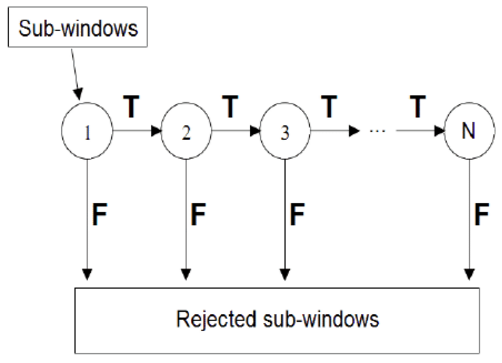
\includegraphics[width=80mm]{Imagenes/deteccion_cascade.png}
		\caption{Detección Cascade.}
		\vspace{0.15cm}
		\textit{Fuente: Evaluation of Haar Cascade Classifiers for Face Detection, OpenCV.}
		\label{fig:deteccion_cascade}
\end{figure} 

\section{Redes Neuronales}
\subsection{Biológicas}

Son el principal elemento del Sistema Nervioso. Las redes neuronales biológicas son el resultado de la union de varias neuronas entrelazadas entre si. Una neurona es una célula compuesta por tres partes fundamentales: el cuerpo, un numero de extensiones llamadas dendritas que sirven de entradas, y una larga extensión llamada axón, la cual se activa como salida. Existe un proceso de comunicacion entre neuronas, el cual es conocido como 'la sinapsis', este proceso conecta el axón de una neurona a las dendritas de las otras neuronas para comunicarse por medio de impulsos electricos. Las neuronas están dispuestas en multiples capas. Por lo general las neuronas de una primera capa reciben entradas desde otra capa y envían sus salidas o impulsos nerviosos a las neuronas de una tercera. Existe un proceso de retroalimentación que se origina cuando los impulsos nerviosos de una neuronal son enviadas a ella misma, originando asi un ciclo donde la imformacion se mantiene por periodos de tiempo. Similar, puede ocurrir la comunicacion entre neuronas de la misma capa.

Las conexiones entre neuronas tienen pesos asociados que representan la influencia de una sobre la otra. Si dos neuronas no están conectadas, el correspondiente peso de enlace es cero. Esencialmente, cada una envía su información de estado multiplicado por el correspondiente peso a todas las neuronas conectadas con ella. Luego
cada una, a su vez, suma los valores recibidos desde sus dendritas para actualizar sus estados respectivos.

Las redes biologicas son entrenadas por medio de la experiencia vivida durante el dia a dia (imagenes recolectadas por el ojo humana y procesadas por el cerebro), de esta forma, estimulando a cada neurona a aprender caracteristicas especiales que ayuden a identificar un determinado objeto. Cabe mencionar que la efectividad y precisión con la que se pueda reconocer un objeto, depende mucho de la cantidad de imagenes previas que se ayan visto sobre este. Además, se producirán respuestas cuando, en la utilización, se presenten entradas totalmente nuevas para el sistema. De este modo el sistema de red neuronal no reside necesariamente en la elegancia de la solución particular sino en su generalidad de hallar solución a problemas particulares, habiéndose proporcionado ejemplos del comportamiento deseado. Esto permite la evolución de los sistemas autómatas sin una reprogramación explicita~\cite{21RedesNeuronales}.

De acuerdo con estudios previos, muchos trabajos orientados al estudio del cerebro humano y la medicina, mencionan que una persona tiene alrededor de $10^{11}$ neuronas, cada una con alrededor de $10^4$ salidas. Donde, la estructura de neuronas de la corteza cerebral es modular: si bien todas las partes del cerebro son relativamente similares, diferentes partes hacen diferentes cosas; a partir de una estructura general, según la experiencia se generan nuevas estructuras especificas al problema a resolver~\cite{16pusiol2014redes}. 


\begin{figure}[H]
		\centering
		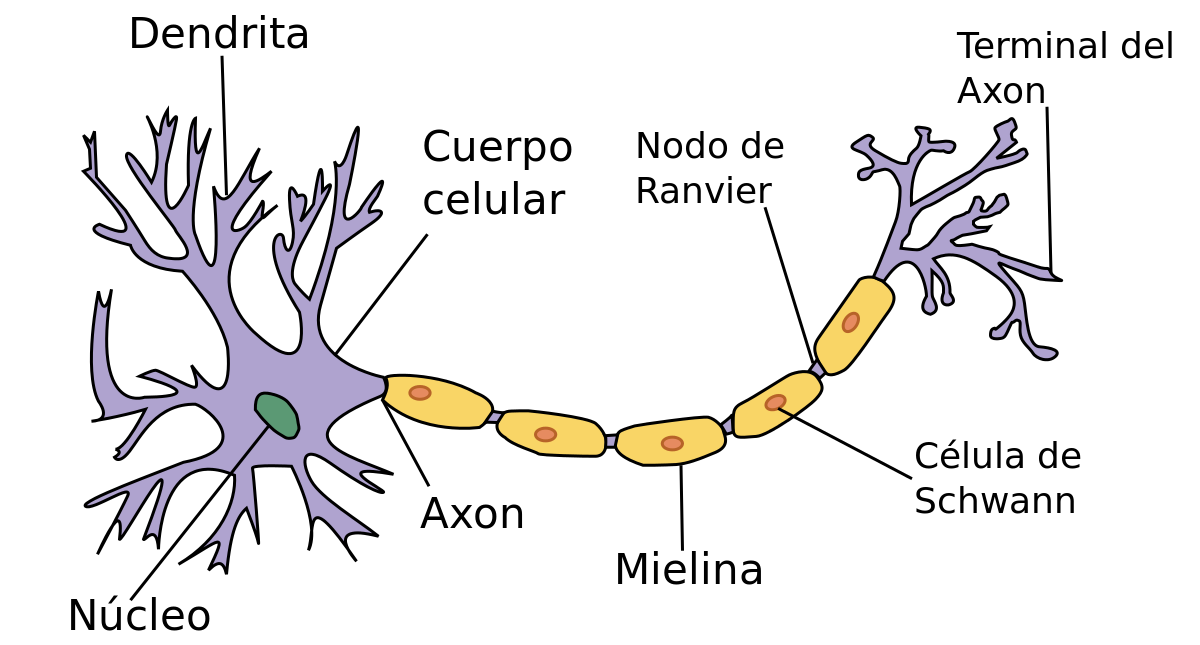
\includegraphics[width=100mm]{Imagenes/neurona_biologica.png}
		\caption{Neurona biológica}
		\vspace{0.15cm}
		\textit{Fuente: Patri Tezanos, Neurociencia, 2016.}
		\label{fig:neurona_biologica}
\end{figure} 


\subsection{Artificiales}
Las Redes Neuronales Artificiales (ANN) imitan el funcionamiento del cerebro, basicamente,  el tipo de  conexiones existentes (ejemplo: las neuronas de una capa previa estan conectadas a neuronas de la siguiente capa), estructura (numero de capas) y transferencia de informacion entre neuronas. Este tipo de arquitectura son aptas para resolver problemas que no poseen un algoritmo claramente definido, transformando asi una entrada en una salida; aprenden, reconocen y aplican relaciones entre objetos. Para realizar este tipo de procesos o tareas, se emplea normalmente un conjunto de ejemplos representativos para 'entrenar' el sistema o la red neuronal (en nuestro caso, imagenes de expresiones faciales), que, a su vez, se adaptan ajustando los pesos de cada neurona de tal manera que pueda producir salidas deseadas a cada imagen de entrada.

Además, similar a las redes neuronales biologicas, se producirán respuestas, cuando en la utilización se presenten entradas totalmente desconocidas por el sistema entrenado. De este modo el sistema de red neuronal artificial no se limita a solo reconocer imagenes que ayan sido previamente vistas, sino en su generalidad para hallar similaridades entre la imagen de entrada y las imagenes previas antes de la fase de entrenamiento, generando asi un sistema robusto capaz de obtener una semejansa enorme a las redes neuronales biologicas.

Las Redes Neuronales Artificiales se basan en el circuito de procesamiento de entradas en el cual los pesos son sumados. Las funciones de peso son conocidas generalmente como atenuadores. En la implementación, las entradas a una neurona son pesadas multiplicando el valor de la entrada por un factor que es menor o igual a uno. El valor de los factores de peso es determinado por el algoritmo de aprendizaje. Las entradas atenuadas son sumadas usando una función no lineal llamada 'Sigmoide'. Si la salida de la función suma excede el valor de entrada máximo de la neurona, esta responde generando una salida. Cada neurona tiene varias entradas y su salida está conectada a un conjunto de otros procesadores de entradas.

Cuando una red funciona en modo normal, a partir de los datos presentados en la entrada, se genera un patrón especifico de salida. La relación entre la entrada y la salida será determinada durante la etapa de  entrenamiento, entonces cuando una entrada conocida es presentada sera dada una salida efectiva. Durante esta etapa de entrenamiento, el algoritmo de aprendizaje ajusta los pesos de las entradas hasta que se alcanza la salida esperada, esto se logra por medio de la minimización de una función de costo(ver ecuación~\ref{eq:funcion_salida}), la cual es representada como la diferencia entre la salida esperada y la salida obtenida.

Devido a la compleja conexión que se realiza entre capas de la red, la complejidad con respecto a terminos computacionales y tiempo de ejecución, puede crecer de manera exponencial. Esto de debe a que cada neurona esta conectada a cientos de neuronas de la siguiente capa y cada neurona de esa siguiente capa realiza lo mismo. Por lo tanto mientras mas sea el numero de capas y neuronas, aparentemente, el sistema sera mejor, pero tambien sera mas complejo y dificil de entrenar.~\cite{21RedesNeuronales}.

La figura~\ref{fig:neurona_artificial} muestra las partes de una neurona artificial, la cual es similar a la estructura de una neurona biologica.

\begin{equation}\label{eq:funcion_salida}
Y_{i} = f(\sum W_{i,j}X{j} - \theta{i})
\end{equation}

\begin{figure}[H]
		\centering
		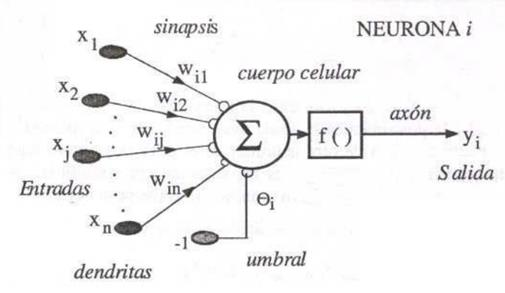
\includegraphics[width=100mm]{Imagenes/neurona_artificial.png}
		\caption{Modelo matemático de una red neuronal}
		\vspace{0.15cm}
		\textit{Fuente: Yuly Cristina Moreira Monserrate, Inteligencia Artificial, 2015.}
		\label{fig:neurona_artificial}
\end{figure}




\section{Arquitectura de una Red Neuronal Artificial}
\subsection{Capas}

\begin{figure}[H]
		\centering
		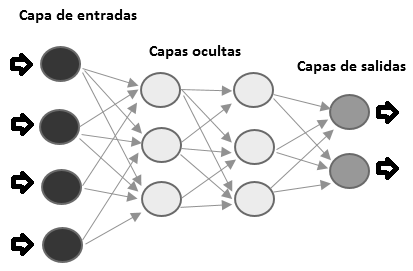
\includegraphics[width=100mm]{Imagenes/capas_red_neuronal.png}
		\caption{Capas de una red neuronal artificial.}
		\vspace{0.15cm}
		\textit{Fuente: Perceptrón multicapa, Wikipedia.}
		\label{fig:capa_red_neuronal}
\end{figure} 

Una red neuronal artificial esta compuesta por tres capas:
\begin{itemize}
\item \textbf{Capa de Entrada.- }Es la encargada de recepcionar los datos de entrada que posteriormente seran procesados. La representacion de estas estradas puede variar dependiendo del tipo de problema que se quiera resolver. En el aso de imagenes, esta se puede representar como una matriz que contiene un determinado valor representativo para cada pixel.
\item \textbf{Capa Oculta.- }Es la encargada de realizar el procesamiento pesado de la informacion, para posteriormente enviar la informacion ya procesada a la capa de salida.
información a la capa de salida.
\item \textbf{Capa de Salida.-} Contiene los resultados como una lista de números. Donde el numero de neuronas de la capa de salida tiene que ser igual al numero de posibles salidad que ofresca el problema a resolver. Otorgando un valor a cada neurona y finalmente, por medio de una funcion de normalizacion obtener la salida definitiva, que corresponde a una sola neurona.  
\end{itemize}


\subsection{Funciones de Activación}
La función de activación es la encargada de mantener los números producidos por cada neurona dentro de una rango razonable(generalmente números reales entre 0 y 1). Esta funcion recibe como entrada la suma de todos los números que llegan por medio de las conexiones entrantes, transforma el valor mediante una determinada funcion y produce un nuevo valor que sera utilizado para la siguiente iteracion. Existen distintas funciones de activacion estudiadas y experimentadas en trabajos previos, donde, algunas de ellas muestran mayor desempeño que las otras.

\begin{itemize}
\item \textbf{Función de activación Sigmoide}

Muchos procesos naturales y curvas de aprendizaje de sistemas complejos muestran una progresión temporal desde unos niveles bajos al inicio, hasta acercarse a un clímax transcurrido un cierto tiempo; la transición se produce en una región caracterizada por una fuerte aceleración intermedia. La función Sigmoide permite describir esta evolución. Su gráfica tiene una típica forma de "S" (ver figura~\ref{fig:funcion_sigmoid}), y esta limitada en el rango de 0 a 1 en el eje de las ordenadas. A menudo la función Sigmoide se refiere al caso particular de la función logística y que viene definida por la ecuación~\ref{eq:funcion_sigmoide}~\cite{24fsigmoide}.

\begin{equation}\label{eq:funcion_sigmoide}
f(x) = \frac{1}{1+\exp^{-x}}
\end{equation}

\begin{figure}[H]
		\centering
		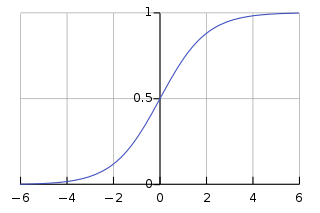
\includegraphics[width=90mm]{Imagenes/fSigmoid.png}
		\caption{Grafica de la función Sigmoide}
		\vspace{0.15cm}
		\textit{Fuente: Sigmoid Function, Wikipedia.}
		\label{fig:funcion_sigmoid}
\end{figure} 

\item \textbf{Función de activación Tangencial}

Es la versión continua de la función signo y se usa en problemas de aproximación. Es importante por sus propiedades analíticas. Es continua a valores en el intervalo [-1,1] (ver figura~\ref{fig:funcion_tang}) e infinitamente diferenciable, Esta función está definida esta definida por la ecuacion~\ref{eq:funcion_tanh}~\cite{25ftangencial}.

\begin{equation}\label{eq:funcion_tanh}
tanh(x) = \frac{\exp^x - \exp^{-x}}{\exp^x + \exp^{-x}}
\end{equation}

\begin{figure}[H]
		\centering
		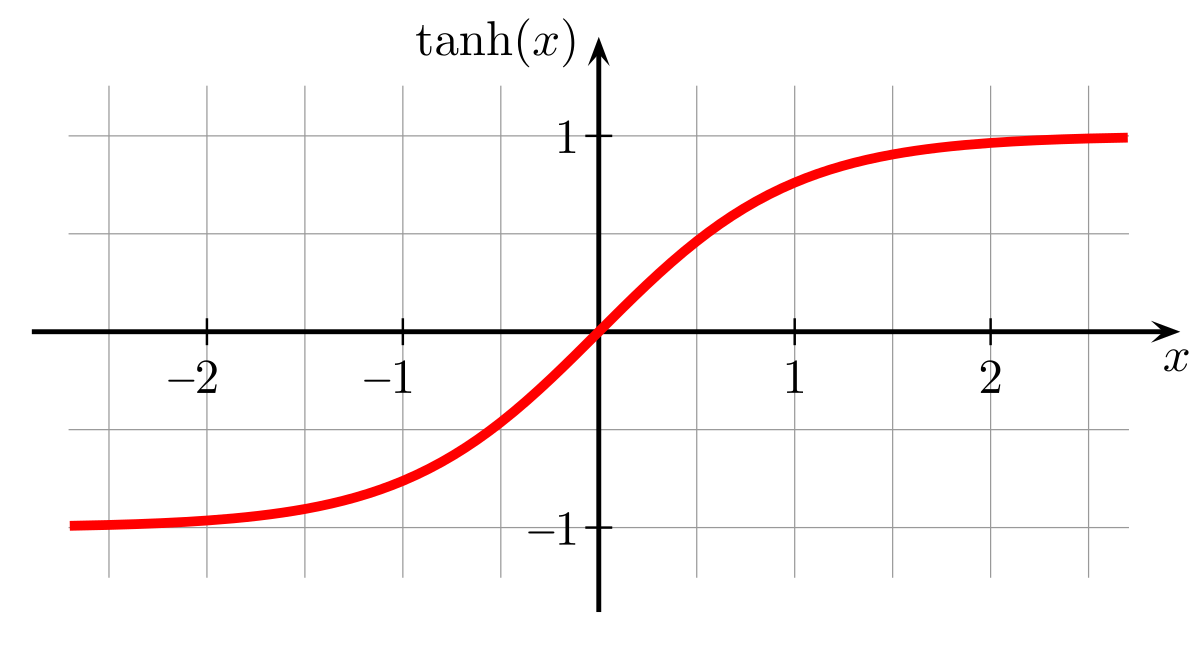
\includegraphics[width=90mm]{Imagenes/fTangent.png}
		\caption{Grafica de la función Tangencial}
		\vspace{0.15cm}
		\textit{Fuente: Tangente hiperbólica, Wikipedia.}
		\label{fig:funcion_tang}
\end{figure} 

\item \textbf{Función de activación RELU (\textit{Rectified Linear Unit})}

Se conoce como una función de rampa y es análoga a la rectificación de onda media. Esta función de activación fue introducida por primera vez a una red dinámica, en un artículo del año 2000, con fuertes motivaciones biológicas y justificaciones matemáticas. Finalmente en el año 2015, despues de ser usada dentro de las redes neuroanles convolucionales, alcanza un gran nivel de eficacia y robustes, superando ampliamente a las funciones de activación logística Sigmoide(la cual esta inspirada en la teoría de probabilidades) y tangente hiperbólica. Siendo asi la mas popular para las Redes Neuronales Profundas. Esta funcion es representada por medio de la ecuación~\ref{eq:funcion_Relu}, y debido a esa ecuación, la parte negativa en el eje abscisas se mantiene en cero, generando la grafica como se muestra en la figura~\ref{fig:funcion_relu}~\cite{26fRelu}.

\begin{equation}\label{eq:funcion_Relu}
f(x)=Max(0,x)
\end{equation}

\begin{figure}[H]
		\centering
		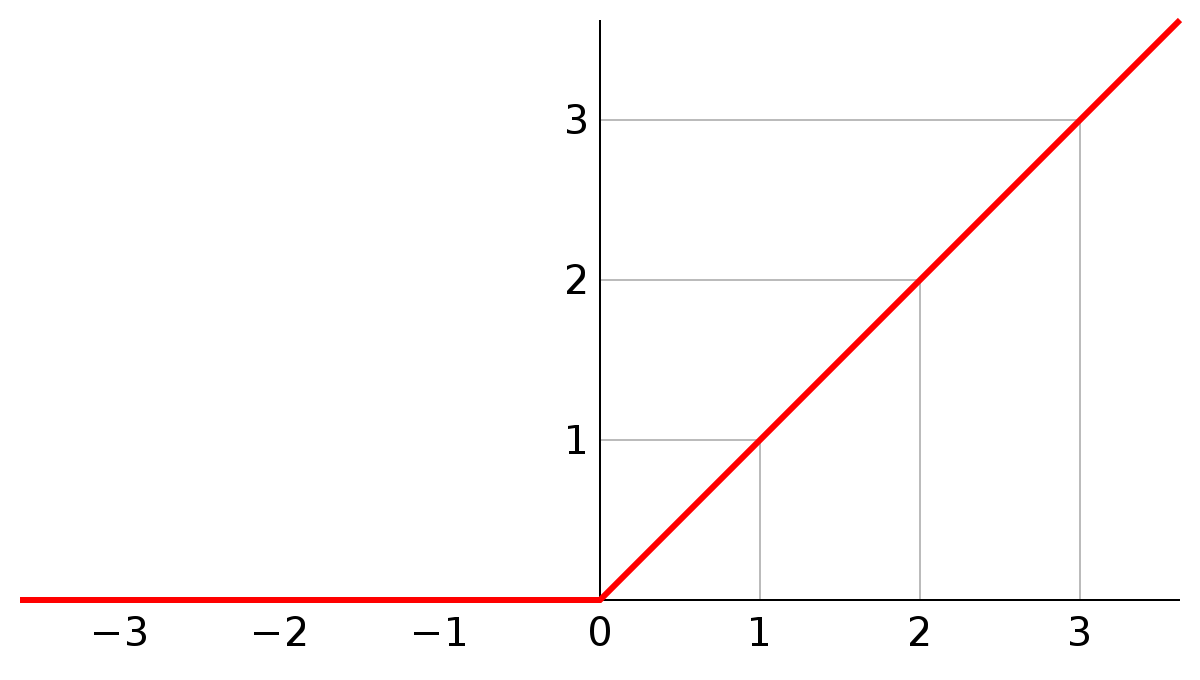
\includegraphics[width=80mm]{Imagenes/fRelu.png}
		\caption{Grafica de la función RELU}
		\vspace{0.15cm}
		\textit{Fuente: Hyperbolic tangent and ReLU neurons, Int8.}
		\label{fig:funcion_relu}
\end{figure} 

\end{itemize}
\subsection{Bias o Sesgo}
Es una cantidad constante que cada neurona de alguna capa oculta añade justo antes de aplicar la función de activacion, este valor puede incrementar o dismunir a la suma de productos(sumatoria de los productos obtenidos despues de multiplicar el valor de cada neurona con su respectivo peso que conecta hacia la siguiente neurona). El objetivo de este valor constante es lograr una convergencia más rápida de la red y evitar que el valor final entrante a una neurona sea un valor muy despreciable o muy significativo. La figura~\ref{fig:arquitectura_red_neuronal} muestra como este valor es intergado en la arquitectura de una red neuronal.


\begin{figure}[H]
		\centering
		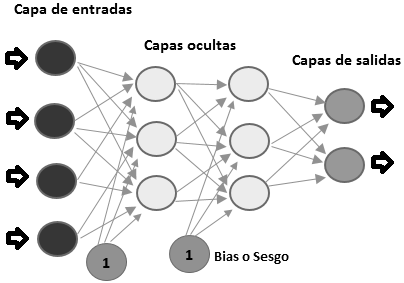
\includegraphics[width=100mm]{Imagenes/arquitectura_red_neuronal.png}
		\caption{Arquitectura de un RNA incluida el sesgo}
		\vspace{0.15cm}
		\textit{Fuente: Propio}
		\label{fig:arquitectura_red_neuronal}
\end{figure}

\section{Implementación de una Red Neuronal Artificial}
Una forma sencilla de implementar redes neuronales, consiste en almacenar los pesos en matrices. Se considera que la red neuronal es un grafo y simplemente representamos este grafo por medio de su matriz de adjacencia, donde cada posicion $(i,j)$ almacena el peso entre la neurona $i$ y la neurona $j$. Posteriormente guardamos los valores de todas las neuronas de una determinada capa en un vector, el producto del vector y la matriz de pesos de salida nos da los valores de entrada de cada neurona en la siguiente capa. Después se aplica la función de activación a cada elemento de ese segundo vector, y repetimos el proceso~\cite{21RedesNeuronales}.

La implementación antes mencionada es una idea general de como se podria implementar una red neuronal(no es el unico algoritmo). En la vida real existen distintos tipos de redes neuronales, donde cada una de ellas presenta una implementación diferente, siendo algunas de ellas mas eficientes computacionalmente que otras.

\section{Backpropagation}
El \textit{BackPropagation} es un algoritmo de aprendizaje supervisado que se usa para entrenar redes neuronales artificial, dicho algoritmo se basa en el descenso de gradiente que es un algoritmo de optimización utilizado para determinar los valores de los parámetros (coeficientes) de una función $f$ que minimiza una función de costes. El descenso de gradiente se utiliza mejor cuando los parámetros no pueden ser calculados analíticamente (por ejemplo, usando algebra lineal) y deben ser buscados por un algoritmo de optimización~\cite{27lehr1993backpropagation}.

La figura~\ref{fig:back_propagation} muestra la representación de como el descenso de gradiente trabaja en la busqueda de los mejores parametros para una determinada funcion (ejemplo: sea la function $f(x)=ax+b$, donde los parametros son las constantes $a$ y $b$). El objetivo es alcanzar el circulo central, el cual representa los parametros óptimos buscados. Para alcanzar dicho objetivo se realiza una serie de paso (representados por las rectas trazadas entre cada par de puntos rojos, como se muestra en la figura~\ref{fig:back_propagation}) que sirven para ajustar los parametros de tal forma que poco a poco se acerquen a la funcion objetivo.

El algoritmo de \textit{Backpropagation} es muy intuitivo. Dada una entrada a la red, esta genera una salida, la cual posteriormente es comparada con la salida deseada, consiguiendo asi el primer error de salida (funcion de costo o diferencia entre la salida deseada y la salida obtenida por la red). Seguido, este error es propagado hacia atras, distribuyendo una porcion de dicho error a todas las neuronas de la capa anterior que aportaron para la obtención de la salida alcanzada. Este proceso se repite, capa por capa, hasta que todas las neuronas de la red ayan recibido una porcion del error obtenido. El objetivo de realizar estos pasos, es crear una red cuyos pesos de cada neurona minimizen la funcion de costo, consiguiendo asi un nivel de precision inversamente proporcional al error alcanzado por cada entrada(mientras menos error, mayor sera la precision alcanzada).

\begin{figure}[H]
		\centering
		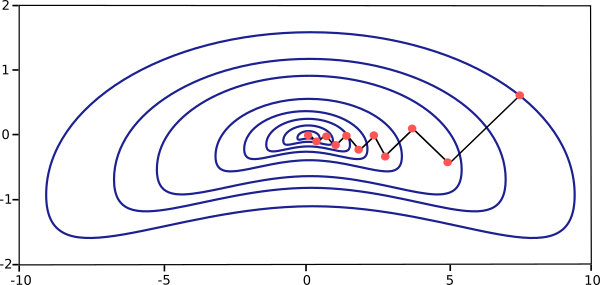
\includegraphics[width=80mm]{Imagenes/back_propagation.png}
		\caption{Descenso de gradiente.}
		\vspace{0.15cm}
		\textit{Fuente: 5 algorithms to train a neural network, Neural Designer.}
		\label{fig:back_propagation}
\end{figure}


\section{Deep Learning}
El \textit{Deep Learning} es un concepto muy amplio, lo que implica que este tenga muchas definiciones. Sin embargo, de una forma muy general, se puede decir que el \textit{Deep Learning} es un concepto que surge de la idea de imitar el cerebro humano por medio de una abstracción mas profunda de las redes neuronales, con el objetivo de crear una inteligencia que mas se asemeje a la inteligencia humana, esta enfoque utiliza una capacidad de abstracción jerárquica, es decir, una representación de los datos de entrada en varios 'niveles'. A diferencia de las Redes Neuronales tradicionales, el \textit{Deep Learning} utiliza multiples capas ocultas para la selección de catacterísticas que son útiles para un mejor aprendizaje; de esta manera, la capa mas profunda dentro de las capas ocultas, obtendrán la representación de características con mayor nivel de abstracción(reconocimiento de lineas, puntos, curvas y otros).

Este enfoque no es mas que un conjunto de algoritmos de \textit{Machine Learning}, que intenta detectar abstracciones de un alto nivel en datos, haciendo uso de arquitecturas compuestas de transformaciones no-lineares multiples~\cite{17bengio2013representation}. Existen varios tipos de aprendizajes, las cuales son tomadas como base para el entrenamiento de una red neuronal en general. Sin embargo, dos principales categorías son resaltadas por las arquitecturas profundas (como se muestra en la figura~\ref{fig:aprendizajes}):

\begin{figure}[H]
		\centering
		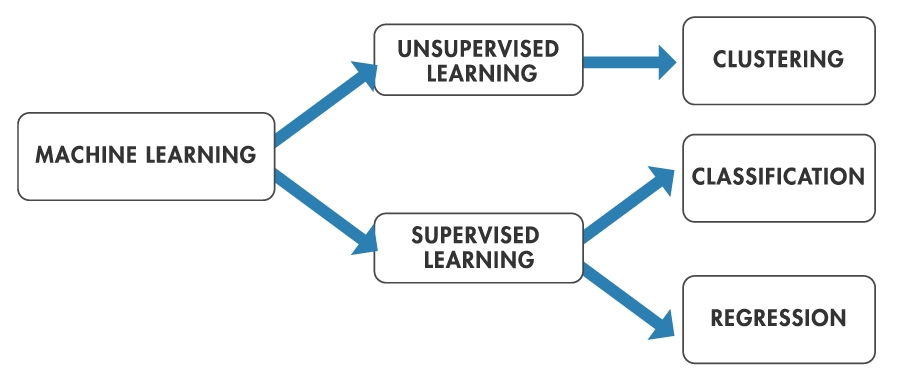
\includegraphics[width=130mm]{Imagenes/aprendizaje_tipos.jpg}
		\caption{Tipos de aprendizaje.}
		\vspace{0.15cm}
		\textit{Fuente: Big Data with MATLAB, Math Works.}
		\label{fig:aprendizajes}
\end{figure}

\begin{itemize}
\item \textbf{Supervisado: } Se caracteriza porque su entrenamiento es controlado por un agente
externo. Es decir, este agente externo guia el entrenamiento de la red mediante una comparacion entra la salida esperada y la salida obtenida por medio de la red. En otras palabras, para realizar este proceso, la base de datos a entrenar necesita contener un campo que indique la salida que se espera por cada dato de entrada. Por ejemplo, sea una arquitectura dedicada a la reconocimiento y clasificacion de numeros en imagenes, entonces, cada vez que pasemos una imagen como entrada a la red, esta imagen debera ir acompañada de una etiqueta que indique cual es el numero que se esta pasando~\cite{18restrepo2015aplicacion}.

\begin{figure}[H]
		\centering
		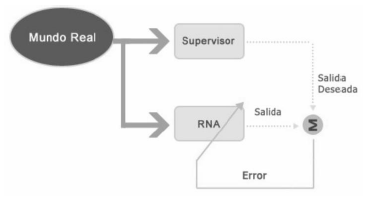
\includegraphics[width=75mm]{Imagenes/grafico_supervisado.png}
		\caption{Aprendizaje supervisado.}
		\vspace{0.15cm}
		\textit{Fuente: López S, Jesús A. Caicedo B, Eduardo F.}
		\label{fig:grafico_supervisado}
\end{figure}



\item \textbf{No supervisado: }
Este enfoque sugiere que el aprendizaje sea realizado presentándole a la red los datos directamente, es decir, ahora no existe un agente externo, campo o etiqueta que indique a la red cuales son los datos que se le proporciona como entrada. La red aprende de ellos, agrupandolos de acuerdo a la similaridad de sus caracteristicas, en algunos casos se realiza este tipo de agrupacion de forma probabilística~\cite{18restrepo2015aplicacion}.

\begin{figure}[H]
		\centering
		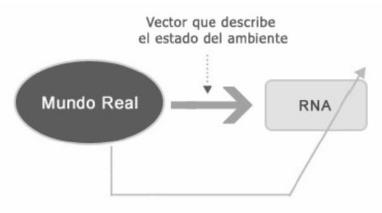
\includegraphics[width=75mm]{Imagenes/grafico_no_supervisado.png}
		\caption{Aprendizaje no supervisado.}
		\vspace{0.15cm}
		\textit{Fuente: López S, Jesús A. Caicedo B, Eduardo F.}
		\label{fig:grafico_no_supervisado}
\end{figure}

\item \textbf{Híbrido: }
Algunas redes tienden a utilizar ambos tipos de aprendizaje para su fase de entrenamiento, ya sea comenzando por un pre-entrenamiento supervisado y finalizando con uno no supervisado o viceversa. Este enfoque se sigue con el objetivo de logran un mejor ajuste, disminuyendo el tiempo de convergencia y entre otras funcionalidades~\cite{18restrepo2015aplicacion}.
\end{itemize}

\section{Redes mas Comunes Consideradas dentro del Deep Learning}
\subsection{Autoencoder}
Es un tipo de Red Neuronal Artificial utilizada para el aprendizaje no supervisado de codificaciones eficientes. El objetivo de una autoencoder es aprender una representación (codificación) para un conjunto de datos, típicamente con el propósito de reducción de dimensionalidad. Recientemente, el concepto autoencoder se ha vuelto más ampliamente utilizado para el aprendizaje de modelos generativos de datos~\cite{28fAutoencoder}.

Un auto-codificador, o autoencoder, aprende a producir a la salida exactamente la misma información que recibe a la entrada. Por eso, las capas de entrada y salida siempre deben tener el mismo número de neuronas. Por ejemplo, como se muestra en la figura~\ref{fig:autoencoder}, si la capa de entrada recibe los píxeles de una imagen, se espera que la red aprenda a producir en su capa de salida exactamente la misma imagen que ha sido introducido~\cite{18restrepo2015aplicacion}.

\begin{figure}[H]
		\centering
		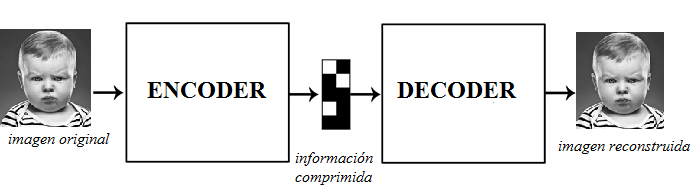
\includegraphics[width=150mm]{Imagenes/autoenconder.png}
		\caption{Arquitectura de una red neuronal Auto-encoder.}
		\vspace{0.15cm}
		\textit{Fuente: Propio.}
		\label{fig:autoencoder}
\end{figure}

\subsection{Redes Neuronales Recurrentes}
Las Redes de Neuronas Recurrentes (\textit{Recurrent Neural Networks}) no tienen una estructura de capas definida, sino que permiten conexiones arbitrarias entre todas las neuronas, incluso creando ciclos. Esto permite incorporar a la red el concepto de temporalidad, y permite que la red tenga memoria, porque los números que introducimos en un momento dado en las neuronas de entrada son transformados, y continúan circulando por la red incluso después de cambiar los números de entrada por otros diferentes~\cite{18restrepo2015aplicacion}.

Este tipo de redes, debido a la capacidad de retener informacion por cortos periodos de tiempo, es altamente utilizado en trabajos relacionados con el procesamiento y analisis de videos, donde las entradas a la red son un conjunto de frames(imagenes), siendo cada imagen la continuacion de la anterior. Sin embargo, similar a las otras redes neuronales, la complejidad en teminos de tiempo de ejecucion(entrenamiendo de la red) sigue siendo una limitacion para experimentar con dichos trabajos, ya que el numero de parametros a optimizar siguen siendo miles de miles, debido a las multiples conexiones que se presentan entre neuronas.  


\begin{figure}[H]
		\centering
		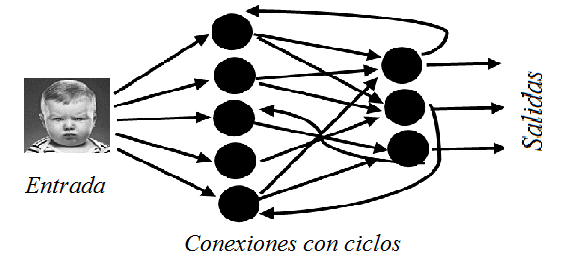
\includegraphics[width=130mm]{Imagenes/red_recurrente.png}
		\caption{Arquitectura de una red neuronal Recurrente.}
		\vspace{0.15cm}
		\textit{Fuente: Propio.}
		\label{fig:red_recurrente}
\end{figure}

\subsection{Redes Neuronales Convolucionales}
Las Redes Neuronales Convolucionales (\textit{Convolution Neural Network}) a diferencia de las Redes Neuronales Recurrentes, mantienen el concepto de capas, pero cada neurona de una capa no recibe conexiones entrantes de todas las neuronas de la capa anterior, sino sólo de algunas. Esto favorece que una neurona se especialice en una región de la lista de números de la capa anterior, y reduce drásticamente el número de pesos y de multiplicaciones necesarias. Lo habitual es que dos neuronas consecutivas de una capa intermedia se especialicen en regiones solapadas de la capa anterior~\cite{16pusiol2014redes}.

Muy diferente del esquema tradicional de las Redes Neuronales Artificiales, estas redes presentan una gran variedad de tipos de capas, donde cada una de ellas tiene una función específica y esta puede repetirse mas de una vez. La siguiente sección sera dedicada a describir con mayor detalles la arquitectura modelo de una Red Neuronal Convolucional.

\section{Arquitectura de una Red Neuronal Convolucional}

Las Redes Neuronales Convolucionales son una estructura compuesta de varias fases entrenables, aprendiendo de cada una de las características con diferentes grados de abstracción. La entrada y salida de cada una de estas etapas son conjunto de arreglos llamados mapas de características, a la salida cada mapa de características representa una característica particular extraída de la imagen de entrada. Cada fase generalmente está compuesta por tres capas: Convolucion, función no lineal y una capa de sub-muestreo. Las ultimas capas por lo general son un conjunto de capas totalmente conectadas.

Una típica arquitectura de Red Neuronal Convolucional para clasificación supervisada está basada en varias etapas(los tres tipos de capas mencionadas en el parrafo anterior: Convolucion y sub-muestreo) seguidas de un clasificador(el conjunto de capas totalmente conectadas). Una de las primeras arquitecturas, es la red propuesta por Yann LeCun(figura~\ref{fig:arquitectura_CNN_Lecun}). Esta red fue utilizada para resolver el problema de reconocimiento de caracteres manuscritos, utilizando una arquitectura con dos fases.


\begin{figure}[H]
		\centering
		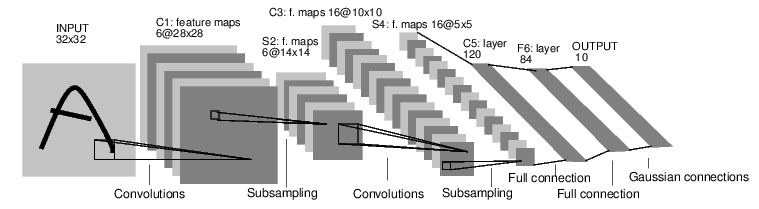
\includegraphics[width=160mm]{Imagenes/arquitectura_CNN_Lecun.png}
		\caption{Arquitectura de una red neuronal Convolucional.}
		\vspace{0.15cm}
		\textit{Fuente: Source: Yann LeCun, 1998.}
		\label{fig:arquitectura_CNN_Lecun}
\end{figure}

Esta red denominada Let-Net, toma una imagen como entrada, la capa siguiente esta constituido por un conjunto de filtros de convolución (mapas de características), seguida por una capa de sub-muestreo encargada de la reduccion de dimensionalidad, seleccionando asi solo los datos mas relevantes. La capa de convolución esta compuesta por seis mapas de características, donde cada uno de ellos no es mas que una matriz con valores asociados. A continuación, se encuentra la capa de sub-muestreo, que, como se menciono antes, agrupa las salidas de las nuevas imágenes originadas por la capa de convolución, generando asi la misma imagen pero con dimensiones menores e información mas relevante. Este nuevo mapa de características sirve de entrada para la siguiente fase dedicada a encontrar características de mayor abstracción. Una cosa importante que cabe resaltar, es que, a medida que se avanza en las fases se aprenden caracteristicas mas relevantes, pero mas invariantes a posicion(por el sub-muestreo). Finalmente, las capas totalmente conectadas se encargan de evaluar las posibles combinaciones de las características aprendidas para lograr clasificar las imágenes dadas~\cite{16pusiol2014redes}.

\subsection{Capa de Convolución}
La capa de convolución es el bloque de construcción básico de una red, esta capa hace la mayor parte del trabajo pesado computacional, debido a que se realizan multiplicaciones de matrices entre la imagen y los filtros de convolución.
\begin{itemize}
\item \textbf{Visión general e intuición sin cerebro.} Los parametros de la capa de convolución consisten en un conjunto de filtros que durante la fase de entrenamiento son aprendidos. Cada filtro es pequeño espacialmente (a lo largo de la anchura y altura), este filtro es aplicado a través de toda la imagen de entrada. Por ejemplo, un filtro típico en una primera capa de una Red Neuronal Convolucional podría tener un tamaño de 5x5x3 (es decir, 5 píxeles anchura y la altura, y 3 ya que las imágenes tienen profundidad 3, los canales de color). Durante el la operacion de convolucion entre el filtro y la imagen de entrada, este se desliza a través del ancho y la altura del volumen de entrada y calcula el productos escalares entre estos dos elementos. A medida que se desplaza el filtro sobre la anchura y la altura del volumen de entrada se produce un mapa de activación de 2 dimensiones que da las respuestas de ese filtro en cada posición espacial. Intuitivamente, la red aprenderá filtros que se activan cuando ven algún tipo de función visual, como un borde en una determinada orientación o una mancha de un cierto color. Después se tendrá todo un conjunto de filtros en cada capa de convolución, y cada uno de ellos va a producir un mapa de activación de 2 dimensiones por separado. Finalmente se apilan estos mapas de activación a lo largo de la dimensión de la profundidad y producen el volumen de salida.~\cite{22RedesNeuronalesConvolu}.

\item \textbf{La vista del cerebro.} Cada entrada en el volumen de salida 3D también se puede interpretar como una salida de una neurona que mira sólo una pequeña región en los parámetros de entrada y comparte con todas las neuronas de la izquierda y derecha (ya que todos estos números resultaría de aplicar el mismo filtro).~\cite{22RedesNeuronalesConvolu}.

\item \textbf{Conectividad local.} Cuando se trata de entradas de alta dimensión como las imágenes, como se vio anteriormente, no es práctico conectar neuronas a todas las neuronas en la capa anterior. En su lugar, se va a conectar cada neurona a sólo una región local del volumen de entrada. La extensión espacial de esta
conectividad es un hiperparámetro llamado campo receptivo de la neurona (equivalente al tamaño del filtro). La extensión de la conectividad a lo largo del eje de profundidad es siempre igual a la profundidad del volumen de entrada. Es importante destacar nuevamente esta asimetría en cómo tratamos las dimensiones espaciales (anchura y altura) y la dimensión de la profundidad: Las conexiones son locales en el espacio (a lo largo del ancho y la altura), pero siempre llenas a lo largo de toda la profundidad del volumen de entrada~\cite{22RedesNeuronalesConvolu}.


\begin{figure}[H]
		\centering
		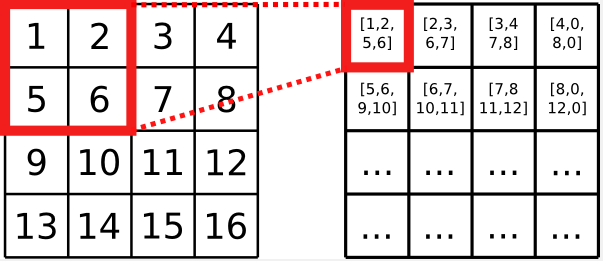
\includegraphics[width=100mm]{./Imagenes/convolucion.png}
		\caption{Ejemplo de convolución con un filtro de dimensiones de 2$\times$2.}
		\vspace{0.15cm}
		\textit{Fuente: Rubén López, Que es y como funciona Deep Learnin.}
        	\label{fig:convolucion}
\end{figure}


\item { \textbf{Pseudo – Codigo.} La representacion de la convolucion por medio de una formula matematica se muestra en la ecuacion~\ref{eq:ecuac_conv}. Los valores de un píxel en la imagen de salida se calculan multiplicando cada valor del kernel por los valores de píxeles de la imagen de entrada correspondientes. Esto se puede describir algorítmicamente con el siguiente pseudo-código:

\begin{equation}\label{eq:ecuac_conv}
V = \frac{\sum^{q1}_{i=0}\sum^{q2}_{i=j} f_{i,j}*k_{i,j}}{F}
\end{equation}

\begin{algorithm}
\caption{Pseudo-Codigo Convolucion\\
La convolucion de una image f(x,y) con un kernel k(x,y) con dimensiones h$\times$w y (2h+1)$\times$(2w+1) respectivamente produce una nueva imagen g(x,y)}\label{alg:euclid}
\begin{algorithmic}[H]
\Procedure{Convolucion}{$f,k$}\Comment{Convolucion de la imagen f con el kernel k}

\For{\texttt{y:=1 to W}}

\For{\texttt{x:=1 to H}}
  \State $sum=0$
     \For{\texttt{i:=-h to h}}
		\For{\texttt{j:=-w to w}}
           \State $sum=sum + k(j,i)*f(x-j,y-i)$
		\EndFor
	 \EndFor 
  \State $g(x,y)=sum$
\EndFor
\EndFor
\State \textbf{return} $g$\Comment{Resultado de la convolucion entre f y k}
\EndProcedure
\end{algorithmic}
\end{algorithm}

Donde:
\begin{itemize}
\item $f_{i,j}$: Corresponde al pixel en la posición $i,j$ de la imagen f respecto al kernel k.
\item $k_{i,j}$: Corresponde al pixel en la posición $i,j$ del kernel k.
\item $q1\times q2 = (2h+1)\times(2w+1)$: Representa las dimensiones del kernel.
\item $F$: Es la suma de los coeficientes del kernel (1 si la suma es igual a 0).
\item $g(i,j)$: Representa el valor de salida del pixel en la posición $i,j$.
\end{itemize}}

\end{itemize}


\subsection{Submuestreo}
Es común insertar periódicamente una capa de agrupación entre capas sucesivas
de convolución en una arquitectura de Red Neuronal Convolucional. Su función es
reducir progresivamente el tamaño espacial de la representación para reducir la cantidad
de parámetros y el cálculo en la red, y por lo tanto también para controlar el sobre ajuste.
La capa de agrupación funciona independientemente en cada segmento de profundidad
de la entrada y la redimensiona espacialmente, utilizando la operación MAX. La forma
más común es una capa de agrupación con filtros de tamaño 2x2 aplicado con una zancada
de 2 muestras descendentes cada porción de profundidad en la entrada por 2 a lo largo
tanto de ancho como de altura, descartando el 75\% de las activaciones. En este caso, cada
operación MAX tomaría un máximo de 4 números (pequeña región 2x2 en una parte de
profundidad). La dimensión de profundidad no cambia. Más generalmente, la capa de
agrupación:

\begin{itemize}
\item Acepta un volumen de tamaño W1xH1xD1
\item Requiere 2 hiperparámetro
  \begin{itemize}
  \item Su extensión espacial F
  \item La zancada S
  \end{itemize}
\item Produce un volumen de tamaño: W2xH2xD2
  \begin{itemize}
  \item $W2 =  \frac{W1 - F}{S + 1}$
  \item $H2 = \frac{H1 - F}{S + 1}$
  
  \item D2 = D1
  \end{itemize}
\item Introduce parámetros cero, ya que calcula una función fija de la entrada.
\item Tiene en cuenta que no es común utilizar cero como relleno para las capas de
agrupación
\end{itemize}

Sólo hay dos variaciones comunes de la capa de agrupación máxima encontrada
en la práctica: Una capa de agrupación con F = 3, S = 2F, S = 2 (también llamada
superposición de agrupación) y más comúnmente F = 2, S = 2F, S = 2 Los tamaños
de agrupación con campos receptivos más grandes son demasiado destructivos~\cite{22RedesNeuronalesConvolu}.

\begin{figure}[H]
		\centering
		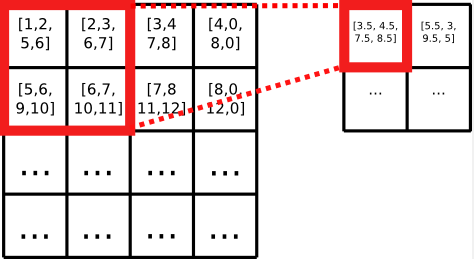
\includegraphics[width=100mm]{./Imagenes/submuestre.png}
		\caption{Ejemplo de Submuestreo con una ventana de 2X2 y calculando el promedio}
		Source: Rubén López, https://rubenlopezg.wordpress.com/2014/05/07/que-es-y-como-funciona-
deep-learning/
        \label{fig:submuestre}
\end{figure}


\subsection{Capa de normalización}
Normalizar las activaciones de la capa anterior en cada lote, es decir, se aplica una
transformación que mantiene la activación de cierre media de 0 y la desviación estándar
de activación cerca de 1~\cite{22RedesNeuronalesConvolu}.

\subsection{Capa totalmente conectada}
Las neuronas en una capa completamente conectada tienen conexiones completas con
todas las activaciones en la capa anterior, como se ve en las redes neuronales regulares.
Por tanto, sus activaciones pueden calcularse con una multiplicación matricial seguida de
un desplazamiento de polarización~\cite{22RedesNeuronalesConvolu}.


\begin{figure}[H]
		\centering
		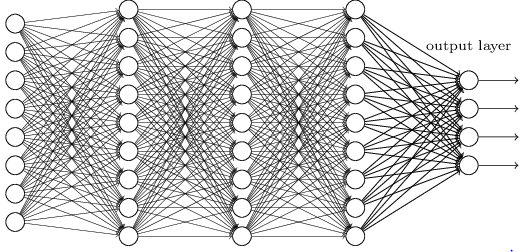
\includegraphics[width=100mm]{./Imagenes/grafico_full_conect.png}
		\caption{Capa totalmente conectada}
		Source: Michael A. Nielsen, http://neuralnetworksanddeeplearning.com/chap6.html
		\label{fig:grafico_full_conect}
\end{figure}

\subsection{Función de normalización(Softmax)}
La regresión softmax es sólo otro nombre para regresión lineal multinomial o
simplemente clase múltiple de regresión logística.

En su esencia, regresión de softmax es una generalización de la regresión logística
que podemos utilizar para la clasificación de clase múltiple (bajo el supuesto de que las
clases son mutuamente excluyentes). En cambio, utilizamos el modelo de regresión
logística (estándar) en tareas de clasificación binario.

\begin{figure}[H]
		\centering
		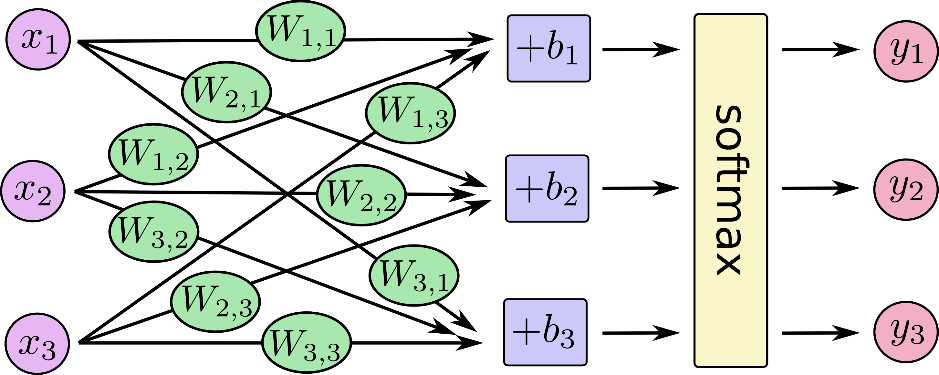
\includegraphics[width=100mm]{./Imagenes/arquitectura_cnn_softmax.png}
		\caption{Arquitectura de una CNN con Softmax}
		Source: Samuel Salvatella, http://ssalva.bitballoon.com/blog/2016-08-30-tensorflow/
		\label{fig:arquitectura_cnn_softmax}
\end{figure}


En las matemáticas , la función softmax , o función exponencial normalizada , es
una generalización de la función logística que permite la utilización de un vector de
dimensión.. La función está dada por

\begin{equation}\label{eq:ecuac_soft}
P(Y = j|Z^i) = \phi_{softmax}(Z^i)= \frac{\exp^{Z^i}}{\sum^k_{j=0}\exp^{Z^{i}_k}}
\end{equation}
Equation \eqref{eq:ecuac_soft} Formula softmax, Donde:\\
$Z = w_{0}x_{0} + w_{1}x_{1} +...+w_{m}x_{m} = \sum_{l=0}^m w_{l}x_{l} = w^Tx$


\section{ENTRENAMIENTO DE UNA RED NEURONAL CONVOLUCIONAL}

El proceso de la CNN para la parte del entrenamiento utiliza el algoritmo
BackPropagation que consiste en calcular una función objetivo que es el de minimizar el
error haciendo para esto la retro propagación del error obtenido a las capas anteriores a la
salida para que se ajusten los pesos de las conexiones entre neuronas.

El algoritmo BackPropagation trabaja de la siguiente forma:

\begin{itemize}
\item Se dan datos de entrada a la red neuronal.
\item Propaga dichas entradas hasta la capa de salida con pesos iniciales definidos o
aleatorios.
\item Calcula el error en la capa de salida.
\item Propaga dicho error hacia las neuronas ocultas (hacia atrás).
\item Cambia los pesos de las conexiones.
\end{itemize}

\section{SOBRE LAS EXPRESIONES FACIALES}
\subsection{Paul Ekman}

Después de que su madre desarrolló una enfermedad mental y se suicidó, Paul
Ekman (psicólogo y científico del comportamiento) dedicó su vida a la Psicoterapia y
ayudar a las personas con trastornos mentales. Él comenzó su investigación en la
comunicación no verbal en la década de 1950, el desarrollo de maneras sistemáticas para
medir el lenguaje corporal. En el proceso, descubrió que, a través de la investigación
empírica, pudo identificar constantemente las expresiones faciales creadas por el
movimiento de los músculos de la cara. Y así, Ekman amplió su investigación para incluir
expresiones faciales y sus significados~\cite{29ekman2016scientists}.


\subsection{Las seis emociones básicas}
Antes de Ekman llegó a la escena, se creía ampliamente (por antropólogos
incluyendo Margaret Mead) que las expresiones faciales y las emociones que ellos
representan se determinaron por la cultura – que las personas aprendieron a hacer y leer
las expresiones faciales de sus sociedades. Ekman se dispuso a probar esta idea en
1968. Él viajó a Papúa Nueva Guinea para estudiar las expresiones faciales de los
miembros de la tribu Fore apartada, donde aprendió que podían identificar
constantemente las emociones en las expresiones faciales por mirar fotos de la gente de
otras culturas, a pesar de que la tribu no había sido expuesta a cualquier exterior culturas.

Se hizo evidente, entonces, que las expresiones faciales son interculturales, su
investigación reveló que existe un conjunto universal de ciertas expresiones faciales se
utilizan tanto en el mundo occidental y oriental. Esta lista de expresiones faciales
universales, que Ekman publicó en el año 1972, dispone de las seis emociones
básicas. Tomar por lo vistazo a la lista, así como imágenes, definiciones y movimientos
musculares de estas emociones, a continuación:

\begin{itemize}
\item {\textbf{Cólera:} 
\begin{itemize}
\item \textbf{Descripción.-} El antagonismo hacia una persona o un objeto a menudo se sentía
después de que usted siente que ha sido agraviado u ofendido.
\item { \textbf{Movimientos musculares faciales.-} La reducción de las cejas, apretar y estrechar
los labios, los ojos mirando, apretando los párpados inferiores, con menos
frecuencia, empujando la mandíbula hacia adelante.

\begin{figure}[H]
		\centering
		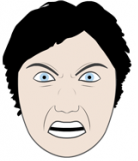
\includegraphics[width=20mm]{./Imagenes/colera.png}
		\caption{Expresión Facial de Cólera}
		Source: Paul Ekman, http://www.serperuano.com/2014/03/paul-ekman-las-6-emociones-basicas/
		\label{fig:colera}
\end{figure}}
\end{itemize}}



\item {\textbf{Felicidad:} 
\begin{itemize}
\item \textbf{Descripción.-} Agradable sensación de satisfacción y bienestar.
\item { \textbf{Movimientos musculares faciales.-} Smiling – tirando hacia arriba comisuras de
la boca, contrayendo los músculos grandes orbitales alrededor de los ojos.

\begin{figure}[H]
		\centering
		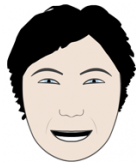
\includegraphics[width=20mm]{./Imagenes/felicidad.png}
		\caption{Expresión Facial de Felicidad}
		Source: Paul Ekman, http://www.serperuano.com/2014/03/paul-ekman-las-6-emociones-basicas/
		\label{fig:felicidad}
\end{figure}}
\end{itemize}}



\item {\textbf{Sorpresa:} 
\begin{itemize}
\item \textbf{Descripción.-} Sensación de malestar o sorpresa ante un hecho inesperado.
\item { \textbf{Movimientos musculares faciales.-} Levantando las cejas altas (que puede causar
arrugas en la frente), abriendo los ojos como platos, dejando caer la mandíbula
tan boca es ágape.

\begin{figure}[H]
		\centering
		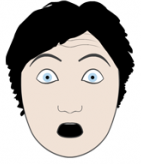
\includegraphics[width=20mm]{./Imagenes/sorpresa.png}
		\caption{Expresión Facial de Sorpresa}
		Source: Paul Ekman, http://www.serperuano.com/2014/03/paul-ekman-las-6-emociones-basicas/
		\label{fig:sorpresa}
\end{figure}}
\end{itemize}}


\item {\textbf{Asco:} 
\begin{itemize}
\item \textbf{Descripción.-} Desagrado intenso o condena causada por algo ofensivo o
repulsiva.
\item { \textbf{Movimientos musculares faciales.-} La reducción de las cejas, curvando el labio
superior, arrugando la nariz.

\begin{figure}[H]
		\centering
		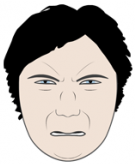
\includegraphics[width=20mm]{./Imagenes/asco.png}
		\caption{Expresión Facial de Asco}
		Source: Paul Ekman, http://www.serperuano.com/2014/03/paul-ekman-las-6-emociones-basicas/
		\label{fig:asco}
\end{figure}}
\end{itemize}}



\item {\textbf{Tristeza:} 
\begin{itemize}
\item \textbf{Descripción.-} Sentimiento de infelicidad o tristeza.
\item { \textbf{Movimientos musculares faciales.-} Los párpados caídos, la reducción de las
esquinas de la boca, labios fruncidos, los ojos bajos.

\begin{figure}[H]
		\centering
		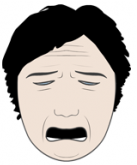
\includegraphics[width=20mm]{./Imagenes/tristeza.png}
		\caption{Expresión Facial de Tristeza}
		Source: Paul Ekman, http://www.serperuano.com/2014/03/paul-ekman-las-6-emociones-basicas/
		\label{fig:tristeza}
\end{figure}}
\end{itemize}}


\item {\textbf{Miedo:} 
\begin{itemize}
\item \textbf{Descripción.-} Sensación de aprehensión provocada por la percepción de peligro,
amenaza o imposición de dolor.
\item { \textbf{Movimientos musculares faciales.-} Levantando las cejas / dibujar las cejas
juntas, tensando los párpados inferiores, que se extiende horizontalmente labios,
la boca ligeramente abierta.

\begin{figure}[H]
		\centering
		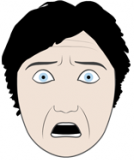
\includegraphics[width=20mm]{./Imagenes/miedo.png}
		\caption{Expresión Facial de Miedo}
		Source: Paul Ekman, http://www.serperuano.com/2014/03/paul-ekman-las-6-emociones-basicas/
		\label{fig:miedo}
\end{figure}}
\end{itemize}}

\end{itemize}


\subsection{Otras expresiones faciales}
Los hallazgos de Ekman sobre las expresiones faciales universales revelaron el
carácter intercultural de la relación entre la comunicación no verbal y la emoción, sin
embargo, las teorías de Ekman han evolucionado desde que ideó su lista de emociones
básicas. En la década de 1990, añadió una serie de otros a la lista de emociones
universales, aunque hizo hincapié en que no todos ellos pueden ser identificados
utilizando expresiones faciales. Estas emociones adicionales son~\cite{29ekman2016scientists}

\begin{itemize}
\item Diversión
\item Desprecio
\item Contentamiento
\item Vergüenza	
\item Emoción
\item Culpa
\item El orgullo de los logros
\item Alivio
\item Satisfacción
\item Placer sensorial
\item Vergüenza
\item Neutro
\end{itemize}
